\section{Implementation}
\label{sec:impl}

%At the end host, \sys requires a reliable transport. The transport can be built over any at-most-once packet transmission interfaces, \textit{e.g.}, UDP, UNIX raw socket, RDMA unreliable datagram~\cite{infinibandrocev2} or netmap~\cite{rizzo2012netmap}. We implement the message transport on the top of a user-mode TCP stack~\cite{dunkels2001design} for loss recovery and congestion control. Beacon packets are sent directly, bypassing the TCP stack. To ensure that retransmitted packets do not violate timestamp monotonicity, we add a TCP option to mark them. In addition, we maintain a mapping from TCP sequence numbers to timestamps, and update commit barrier when a TCP ACK is received.

We implement a reliable transport at the end host to deliver messages. Our implementation is built on the top of a user-mode TCP stack~\cite{dunkels2001design} for loss recovery and congestion control. Beacon packets are sent directly, bypassing the TCP stack. To ensure that retransmitted packets do not violate timestamp monotonicity, we add a TCP option to mark them. In addition, we maintain a mapping from TCP sequence numbers to timestamps, and update commit barrier when a TCP ACK is received.

In the following, we present implementations of in-network processing at three types of network switches with different programming capabilities. 

\begin{figure*}[t]
\centering
\subfloat[Reconfigurable swithing chips.\label{fig:p4}]
{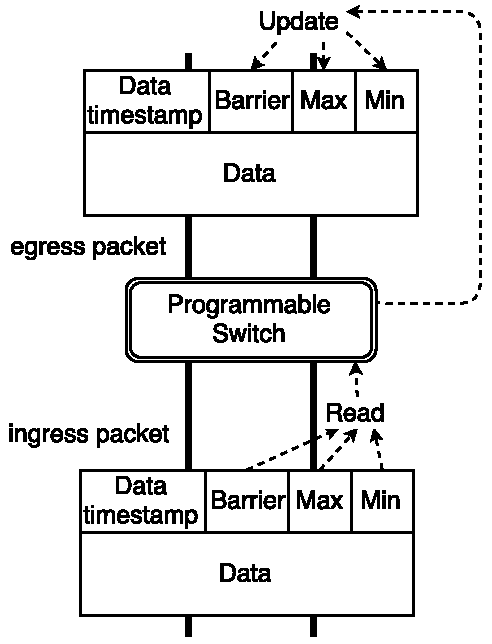
\includegraphics[width=.25\textwidth]{images/p4_implementation.pdf}}
\hspace{0.04\textwidth}
\subfloat[Switch CPU\label{fig:commodity}]
{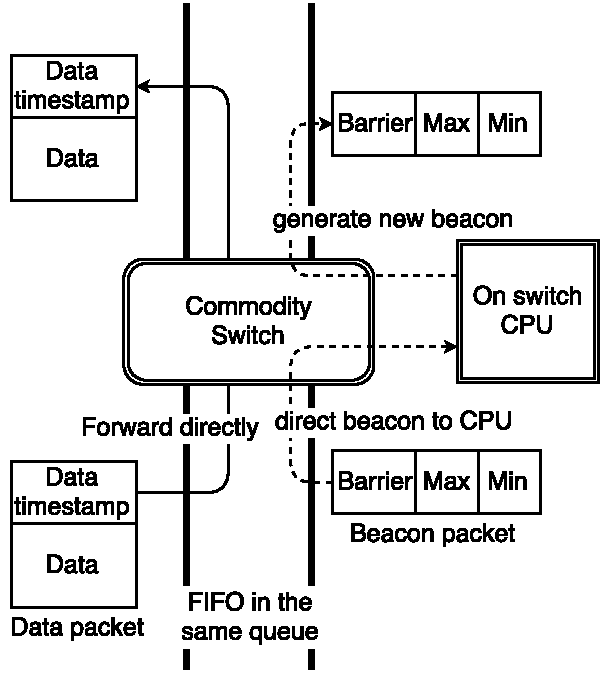
\includegraphics[width=.28\textwidth]{images/commodity_implementation.pdf}}
\hspace{0.04\textwidth}
\subfloat[End hosts only.\label{fig:end-host}]
{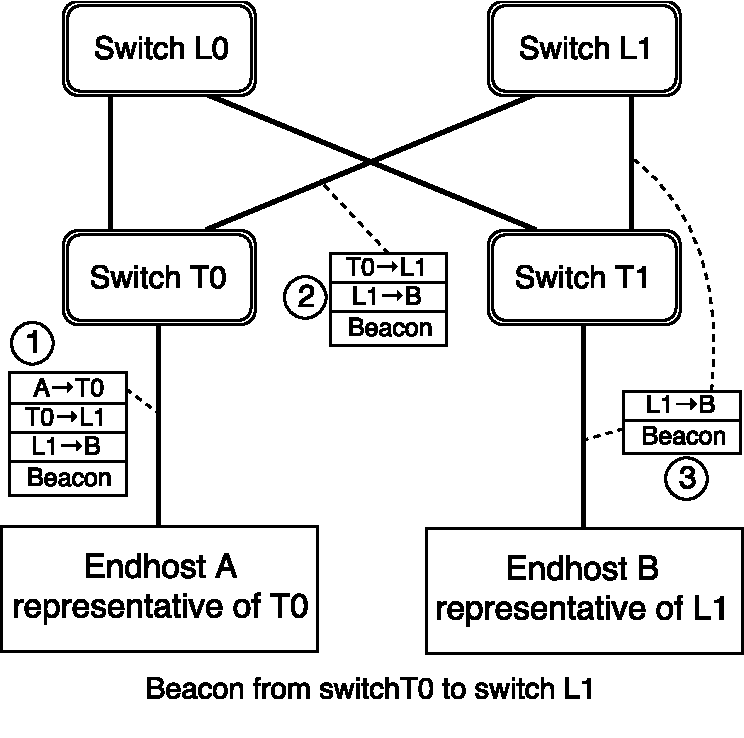
\includegraphics[width=.3\textwidth]{images/endhostonly_implementation.pdf}}
\caption{\sys dataflow in networks with different programming capabilities.}
\label{fig:impl}
\vspace{-1em}
\end{figure*}

\subsection{Reconfigurable Switcing Chips}
\label{sec:p4}
The reconfigurable switching chip is able to maintain a handful of states $\mathcal{S}$ and process each packet $P$ through the state machine $P', \mathcal{S}' = f(P, \mathcal{S})$. Hence, for the switch with a reconfigurable chip, we can implement the in-network processing logics on the chip. 

We choose Barefoot Tofino~\cite{tofino} for the implementation. \sys needs 8 state registers per input link and 5 state registers per output link. Each data packet carry three timestamp fields: message timestamp, unreliable barrier and commit barrier, as well as loss encountered flag (Algorithm~\ref{alg:loss-detection}).
A timestamp is a 6-byte integer, indicating the number of nanoseconds passed on the host. Since the timestamps wrap around in 7.8 hours, we use PAWS~\cite{jacobson1992tcp} to compare timestamps: If $s$ and $t$ are timestamps, $s < t$ if and only if $0 < t - s < 2^{47}$, computed in 48-bit unsigned arithmetic. As shown in Figure~\ref{fig:p4}, the beacon packets carry not only the same set of timestamps and flag as data packets, but also information for minimax clock synchronization (Algorithm~\ref{alg:minimax}).

\subsection{Switch CPU}
\label{sec:commodity}

For the switch, \textit{e.g.,} Arista DCS-7060CX-32S without a reconfigurable switching chip, we can implement our in-network processing logics using the switch CPU. 
%Data-plane programmable switches are currently not widely available in data centers.
%Although commodity switches cannot process packets in data plane, they have a CPU to process control-plane packets, analogous to directly connecting a server to a port of the switch.
Compared to server CPUs and NICs, the switch CPU is typically less powerful (\textit{e.g.}, 4 cores at 1~GHz) and has lower bandwidth (\textit{e.g.}, 1 Gbps).

Because the CPU cannot process every data packet, as shown in Figure~\ref{fig:commodity}, data packets are forwarded by the switching chip as if there were no \sys service, and stored in reorder buffer on end-host receivers.
The CPU sends beacons periodically on each output link, regardless of whether the link is idle or busy.
Because data and beacon packets are FIFO in switch queues and on network links, the barrier property is preserved. On receivers, buffered data packets are delivered to the application according to barriers in beacon packets.

Compared with the reconfigurable switching chip, this approach slacks the barriers in two aspects.
First, the barriers are updated by periodical beacons instead of by every packet.
Second, the processing delay of beacon packets in switch CPU is longer than the processing delay of data packets by switching chip.
Consequently, the additional reordering delay is (processing delay $\times$ number of hops + beacon interval).

\subsection{Delegate Switch Processing to a Host}
\label{sec:end-host}

In case that the switch vendor does not expose access interfaces to switch CPUs, we can offload the beacon processing to end hosts. The challenge is to maintain the FIFO property.
Beacons with barrier timestamps on a network link $L$ must pass through $L$.
To this end, we designate an \textit{end-host representative} for each network switch.
The location of the representative is arbitrary and does not need to be unique.

As shown in Figure~\ref{fig:end-host}, for two directly connected switches $S_1, S_2$ and their representatives $H_1, H_2$, beacon packets from $H_1$ to $H_2$ need to go through the link $S_1 \rightarrow S_2$.
A beacon packet $H_1 \rightarrow H_2$ is sent with three layers of IP headers: $H_1 \rightarrow S_1$, $S_1 \rightarrow S_2$ and $S_2 \rightarrow H_2$.
We install tunnel termination rules in each network switch to decapsulate one layer of IP header, so the beacon packet will traverse through $H_1 \rightarrow S_1 \rightarrow S_2 \rightarrow H_2$.

Compared with previous section, the delay overhead of delegating a switch to an end-host representative is the RTT from the host to the switch.
